\documentclass{article}

\usepackage{arxiv}

\usepackage[utf8]{inputenc} % allow utf-8 input
\usepackage[T1]{fontenc}    % use 8-bit T1 fonts
\usepackage{lmodern}        % https://github.com/rstudio/rticles/issues/343
\usepackage{hyperref}       % hyperlinks
\usepackage{url}            % simple URL typesetting
\usepackage{booktabs}       % professional-quality tables
\usepackage{amsfonts}       % blackboard math symbols
\usepackage{nicefrac}       % compact symbols for 1/2, etc.
\usepackage{microtype}      % microtypography
\usepackage{graphicx}

\title{R in Trust - A Case study of SARS-CoV2 Open Data Repositories}

\author{
    Nathanael Sheehan
   \\
    College of Engineering, Mathematics and Physical Sciences \\
    Exeter University \\
  University of Exeter, St Germans Road, EX4 7HD Exeter, UK \\
  \texttt{\href{mailto:ns651@exeter.ac.uk}{\nolinkurl{ns651@exeter.ac.uk}}} \\
   \And
    Sabina Leonelli
   \\
    EGENIS, Centre For The Study Of Life Sciences \\
    Exeter University \\
  University of Exeter, St Germans Road, EX4 7HD Exeter, UK \\
  \texttt{\href{mailto:s.leonelli@exeter.ac.uk}{\nolinkurl{s.leonelli@exeter.ac.uk}}} \\
  }


% tightlist command for lists without linebreak
\providecommand{\tightlist}{%
  \setlength{\itemsep}{0pt}\setlength{\parskip}{0pt}}



\begin{document}
\maketitle


\begin{abstract}
In this paper I aruge on the importance of TRUST
\end{abstract}

\keywords{
    SARS-CoV2
   \and
    Open Science
   \and
    Data Governance
  }

\hypertarget{introduction}{%
\section{Introduction}\label{introduction}}

Open Science has transformed the classical modus operandi of scientific
knowledge accumulation and dissemination. The pandemic highlighted the
necessity for rapid, scalable and open access to the latest research
findings, treatments and protocols on the cornavirus. Now exists
hundreds of thousands data repsotiores storing data on the biological
enitity Data repostiores have been buuilt by Governments, univieristies,
busisinerses and publics The greatest example of this has been the
sharing of SARS genomic data, where millions of genomes have been shared
across the world During the Pandemic an open letter was written by the
EBI in support in complete openness in genome sharing and asked for
people to donate all data to a traid of databases Many public figures
and institutions supported the letter saying that coivd was bigger than
all of us, and we must come together Others critiseied the letter and
argued that there database was a wolf in open source clothing and missed
the point in resonsibility for data sharing

This shift in research practice - in conjunction with decreasing costs
in data storage - has led to an exponential increase in ``big'' data and
public repositories that stores such data. This new found importance for
data repostiores mea

TRUSt is a set of principles for data repositiores owners to adhere to
so the community is served and they demonstate the ability to mananage
the data they hold T = transparancey U = User focus, S = Sustainablity,
T = Trust R = Adhering to the designated community's metadata and
curation standards, along with providing stewardship of the data
holdings e.g.~technical validation, documentation, quality control,
authenticity protection, and long-term persistence.

Providing data services e.g.~portal and machine interfaces, data
download or server-side processing.

Managing the intellectual property rights of data producers, the
protection of sensitive information resources, and the security of the
system and its content. The FAIR Data Principles3 highlight the need to
embrace good practice by defining essential characteristics of data
objects to ensure that data are reusable by humans and machines The Open
Archival Information System (OAIS) reference model4 provides
recommendations on setting up archives delivering long-term preservation
of and access to information (in particular, digital information) and
creating preservation packages. None of these encapsulate trust and
tremporal demand that trust takes to build and serve a community
{[}trust table {]}

To start I document my expereince joining each community and
qualiotaitely narrate me expereince conceptaulising the R principles in
each repo I then systhensis the datasets into aggreated months and
explore statistical trends in each dataset I conclusde by a final
discourse on how

\hypertarget{methods}{%
\section{Methods}\label{methods}}

\begin{figure}
\centering
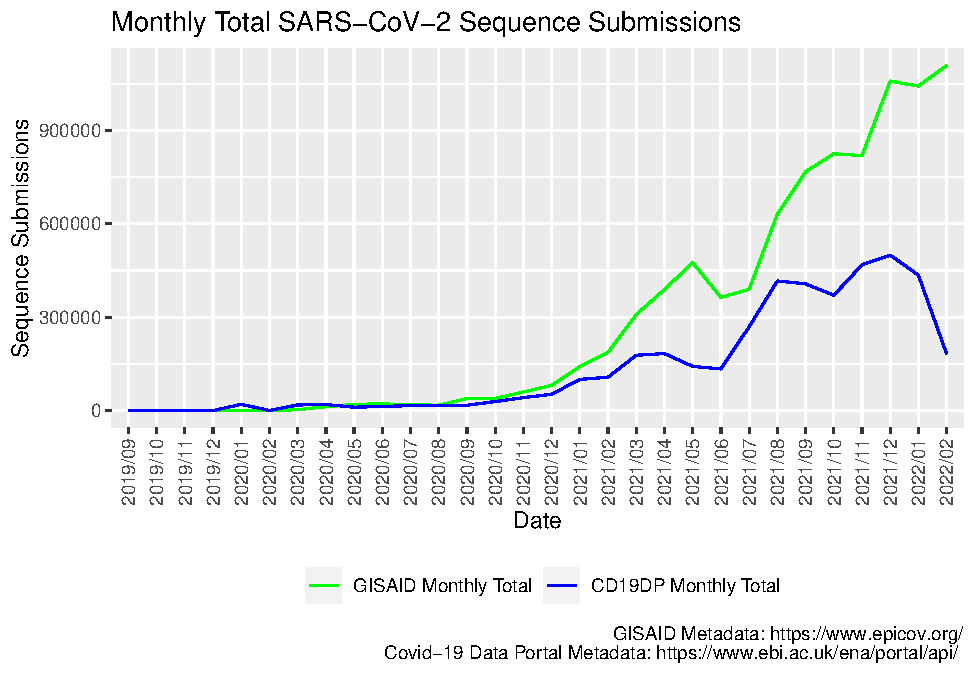
\includegraphics{Report_files/figure-latex/fig2-1.pdf}
\caption{Monthly totals of global SARS-CoV-2 cases sequenced and shared
on the GISAID and Covid-19 Data Platform database until Febuary 22 2022}
\end{figure}

\hypertarget{gisiad}{%
\subsection{GISIAD}\label{gisiad}}

In May of 2008 the Global Initiative on Sharing All Influenza Data
(GISAID) was launched in tandem with the Sixty-first World Health
Assembly. GISAID From its inceptions GISAID was built to be an
alternative to the classical public domain sharing model as it took into
account the beliefs of Member states by providing an accessible database
designed by scientists for scientists.

\hypertarget{covid-19-data-platform}{%
\subsection{COVID-19 Data Platform}\label{covid-19-data-platform}}

\hypertarget{discussion}{%
\section{Discussion}\label{discussion}}

\hypertarget{conclusion}{%
\section{Conclusion}\label{conclusion}}

\bibliographystyle{unsrt}
\bibliography{references.bib}


\end{document}
